\documentclass[journal,12pt,onecolumn]{IEEEtran}
\usepackage{cite}
\usepackage{graphicx}
\usepackage{amsmath,amssymb,amsfonts,amsthm}
\usepackage{algorithmic}
\usepackage{textcomp}
\usepackage{xcolor}
\usepackage{txfonts}
\usepackage{listings}
\usepackage{enumitem}
\usepackage{mathtools}
\usepackage{gensymb}
\usepackage{comment}
\usepackage[breaklinks=true]{hyperref}
\usepackage{tkz-euclide} 
\usepackage{caption}
\usepackage{listings}
\usepackage{gvv}                                        
\usepackage[latin1]{inputenc} 
\usetikzlibrary{arrows.meta, positioning}
\usepackage{xparse}
\usepackage{color}                                            
\usepackage{array}                                            
\usepackage{longtable}                                       
\usepackage{calc}                                             
\usepackage{multirow}
\usepackage{multicol}
\usepackage{hhline}                                           
\usepackage{ifthen}                                           
\usepackage{lscape}
\usepackage{tabularx}
\usepackage{array}
\usepackage{float}
\newtheorem{theorem}{Theorem}[section]
\newtheorem{problem}{Problem}
\newtheorem{proposition}{Proposition}[section]
\newtheorem{lemma}{Lemma}[section]
\newtheorem{corollary}[theorem]{Corollary}
\newtheorem{example}{Example}[section]
\newtheorem{definition}[problem]{Definition}
\newcommand{\BEQA}{\begin{eqnarray}}
\newcommand{\EEQA}{\end{eqnarray}}
\usepackage{float}
\theoremstyle{remark}
\usepackage{circuitikz}
\usepackage{tikz}\title{}
\title{\Huge MN:MINING ENGINEERING}
\author{Vaishnavi Ramkrishna Anantheertha-EE25BTECH11059}
\begin{document}
\maketitle

\section*{Q.1--Q.25 carry one mark each}
\begin{enumerate}
\item ``From where are they bringing their books? \_\_\_\_\_ bringing \_\_\_\_\_ books from \_\_\_\_\_,''

The words that best fill the blanks in the above sentence are  

\begin{enumerate}[label=(\Alph*)]
    \item Their, they're, there
    \item They're, their, there
    \item There, their, they're
    \item They're, there, there
\end{enumerate}
\item ``A \_\_\_\_\_\_ investigation can sometimes yield new facts, but typically organized ones are more successful.''  

The word that best fills the blank in the above sentence is  
\hfill\brak{GATE\ MN\ 2018}
\begin{multicols}{4}
\begin{enumerate}
\item  meandering 
\item  timely
\item consistent
\item systematic
\end{enumerate}
\end{multicols}

\item The area of a square is $d$. What is the area of the circle which has the diagonal of the square as its diameter?  

\hfill\brak{GATE\ MN\ 2018}
\begin{multicols}{4}
\begin{enumerate}
    \item $\pi d$
    \item $\pi d^{2}$ \
    \item $\frac{1}{4}\pi d^{2}$  
    \item $\tfrac{1}{2}\pi d$
\end{enumerate}
\end{multicols}
\item What would be the smallest natural number which when divided either by $20$ or by $42$ or by $76$ leaves a remainder of $7$ in each case?

\hfill\brak{GATE\ MN\ 2018}
\begin{multicols}{4}
\begin{enumerate}
\item $3047$
\item $6047$ 
\item $7987$
\item $63487$
\end{enumerate}
\end{multicols}
\item What is the missing number in the following sequence? 
2, 12, 60, 240, 720, 1440,\_\_\_  ,0

\hfill\brak{GATE\ MN\ 2018} 
\begin{multicols}{4}
\begin{enumerate}
\item $2880$
\item $1440$
\item $720$
\item $0$
\end{enumerate}
\end{multicols}
\section*{Q6-Q10 carries two marks}
\item In appreciation of the social improvements completed in a town, a wealthy philanthropist decided to gift Rs $750$ to each male senior citizen in the town and Rs $1000$ to each female senior citizen. Altogether, there were $300$ senior citizens eligible for this gift. However, only $\tfrac{8}{9}$ of the eligible men and $\tfrac{2}{3}$ of the eligible women claimed the gift. How much money (in Rupees) did the philanthropist give away in total?  

\hfill\brak{GATE\ MN\ 2018}
\begin{multicols}{4}
\begin{enumerate}
\item $1,50,000$
\item $2,00,000$ 
\item $1,75,000$
\item $1,51,000$
\end{enumerate}
\end{multicols}
\item If $pqr \ne 0$ and $p^{-x} = \frac{1}{q}, \; q^{-y} = \frac{1}{r}, \; r^{-z} = \frac{1}{p}$, what is the value of the product $xyz$?   

\hfill\brak{GATE\ MN\ 2018}
\begin{multicols}{4}
\begin{enumerate}
\item $-1$ 
\item $\frac{1}{pqr}$ 
\item $1$
\item $pqr$
\end{enumerate}
\end{multicols}
\item In a party, 60\% of the invited guests are male and 40\% are female. If 80\% of the invited
guests attended the party and if all the invited female guests attended, what would be the ratio of males to females among the attendees in the party?


\hfill\brak{GATE\ MN\ 2018}
\begin{multicols}{4}
\begin{enumerate}
\item $2\colon3$
\item $1\colon1$ 
\item $3\colon2$
\item $2\colon1$
\end{enumerate}
\end{multicols}
\item In the figure below, $\angle DEC + \angle BFC$ is equal to
\begin{figure}[H]
  \centering
  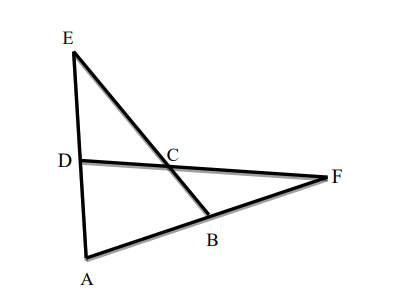
\includegraphics[width=0.4\columnwidth]{figs/angles.png}
  \caption{Triangle}
  \label{fig:angle}
\end{figure}

\hfill\brak{GATE\ MN\ 2018}
  \begin{multicols}{2}
  \begin{enumerate}
    \item $\angle BCD - \angle BAD$
    \item $\angle BAD + \angle BCF$  
    \item $\angle BAD + \angle BCD$
    \item $\angle CBA + \angle ADC$
\end{enumerate}
  \end{multicols}
\item A six sided unbiased die with four green faces and two red faces is rolled seven times.Which of the following combinations is the most likely outcome of the experiment?

\hfill\brak{GATE\ MN\ 2018}
\begin{multicols}{2}
\begin{enumerate}
\item Three green faces and four red faces.
\item Four green faces and three red faces.
\item Five green faces and two red faces.
\item Six green faces and one red face.
\end{enumerate}
\end{multicols}
\end{enumerate}
\begin{enumerate}
\section*{Q1 to Q25 carry one mark eac}
\item \[
\text{If } 
X = \begin{bmatrix}
\cos\theta & \sin\theta \\
-\sin\theta & \cos\theta
\end{bmatrix}, 
\text{ then } XX^{T} \text{ is}
\]
\hfill\brak{GATE\ MN\ 2018}
\begin{enumerate}
\item $ \begin{bmatrix} 0 & 1 \\ 1 & 0 \end{bmatrix}$
\item $\begin{bmatrix} -1 & 0 \\ 0 & -1 \end{bmatrix}$
\item $\begin{bmatrix} 1 & 0 \\ 0 & 1 \end{bmatrix}$
\item $\begin{bmatrix} 0 & -1 \\ -1 & 0 \end{bmatrix}$
\end{enumerate}
\item \text{The values of } x \text{ satisfying the following condition are}
\[
\begin{vmatrix}
4-x & \sqrt{3} \\
\sqrt{3} & 6-x
\end{vmatrix} = 0
\]

\hfill\brak{GATE\ MN\ 2018}
\begin{multicols}{2}
\begin{enumerate}
\item $6,4$ 
\item $4,9$
\item $5,6$
\item $3,7$
\end{enumerate}
\end{multicols}
\item An azimuth of $330^\circ$ corresponds to a quadrant bearing of $N30^\circ W$.

\hfill\brak{GATE\ MN\ 2018}
\begin{multicols}{2}
\begin{enumerate}
  \item $W60^\circ N$
  \item $N30^\circ W$
  \item $S30^\circ W$
  \item $S30^\circ E$
\end{enumerate}
\end{multicols}

 \item Tri-cone drill bit is a type of
\hfill\brak{GATE\ MN\ 2018}
\begin{multicols}{4}
\begin{enumerate}
\item cross bit 
\item button bit
\item rotary roller bit
\item button drag bit
\end{enumerate}
\end{multicols}

\item Exposure of weak roof in junctions of a development district in a coal mine can be decreased by

\hfill\brak{GATE\ MN\ 2018}
\begin{multicols}{2}
\begin{enumerate}
\item increasing dimension of panel barrier
\item stitching side walls
\item increasing support density at junctions
\item staggering the junctions
\end{enumerate}
\end{multicols}

\item The property that CANNOT be determined from uniaxial compressive strength test of a rock sample fitted with strain gauges is

\hfill\brak{GATE\ MN\ 2018}
\begin{multicols}{4}
\begin{enumerate}
\item cohesion
\item Poisson ratio
\item modulus of elasticity
\item dilation
\end{enumerate}
\end{multicols}

\item The radial stress concentration around a long circular tunnel excavated in rock is given by the curve
\begin{figure}[H]
  \centering
  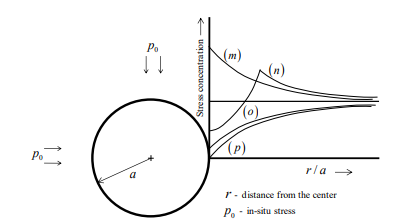
\includegraphics[width=0.4\columnwidth]{figs/dia1.png}
  \caption{The radial stress concentration}
  \label{fig:dai1}
\end{figure}
\begin{multicols}{2}
\begin{enumerate}
\item $m$ 
\item $n$ 
\item $o$
\item $p$
\end{enumerate}
\end{multicols}

\item Ward-Leonard system is provided in the winding system in order to restrict

\hfill\brak{GATE\ MN\ 2018}
\begin{multicols}{2}
\begin{enumerate}
\item over-winding of the cage 
\item deceleration of the cage
\item acceleration of the cage  
\item over-speeding of the cage
\end{enumerate}
\end{multicols}

\item The equipment NOT related to extraction of coal from longwall face operation is

\hfill\brak{GATE\ MN\ 2018}
\begin{multicols}{4}
\begin{enumerate}
\item AFC
\item road header
\item powered support
\item DERD shearer
\end{enumerate}
\end{multicols}
\item The correct figure depicting the extraction of contiguous seams in bord and pillar working is indicated by

\hfill\brak{GATE\ MN\ 2018}

\begin{multicols}{4}
\begin{enumerate}
\item \begin{figure}[H]
  \centering
  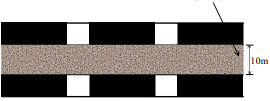
\includegraphics[width=1\columnwidth]{figs/opta.png}
  \caption{Option A}
  \label{fig:opta}
\end{figure}
\item \begin{figure}[H]
  \centering
  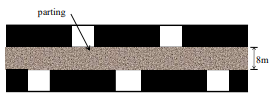
\includegraphics[width=1\columnwidth]{figs/optb.png}
  \caption{Option B}
  \label{fig:optb}
\end{figure}
\item \begin{figure}[H]
  \centering
  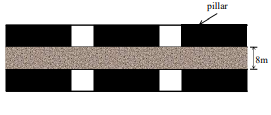
\includegraphics[width=1\columnwidth]{figs/optc.png}
  \caption{Option C}
  \label{fig:optc}
\end{figure}
\item \begin{figure}[H]
  \centering
  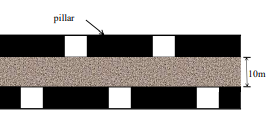
\includegraphics[width=1\columnwidth]{figs/optd.png}
  \caption{Option D}
  \label{fig:optd}
\end{figure}
\end{enumerate}
\end{multicols}
\item The significance of potentially explosive mixture in Coward flammability diagram is 

\hfill\brak{GATE\ MN\ 2018}
\begin{enumerate}
\item \begin{figure}[H]
  \centering
  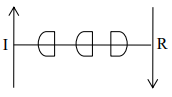
\includegraphics[width=0.2\columnwidth]{figs/A.png}
  \caption{Option A}
  \label{fig:a}
\end{figure}
\item \begin{figure}[H]
  \centering
  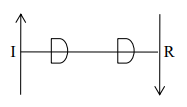
\includegraphics[width=0.2\columnwidth]{figs/B.png}
  \caption{Option B}
  \label{fig:b}
\end{figure}
\item \begin{figure}[H]
  \centering
  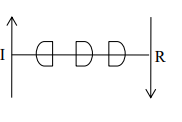
\includegraphics[width=0.2\columnwidth]{figs/C.png}
  \caption{Option C}
  \label{fig:c}
\end{figure}
\item  \begin{figure}[H]
  \centering
  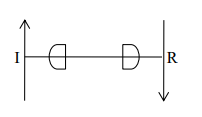
\includegraphics[width=0.2\columnwidth]{figs/D.png}
  \caption{Option D}
  \label{fig:d}
\end{figure}
\end{enumerate}
\item From a coal seam of a mine $1000$ tonnes of coal is produced per day. The seam has inflammable gas emission rate of $14000$ $m^{3}$ per day. Percentage of inflammable gas in general body of air is $0.14$. The gassiness of the seam is

\hfill\brak{GATE\ MN\ 2018}
\begin{multicols}{4}
\begin{enumerate}
\item Degree IV
\item Degree III
\item Degree II
\item Degree I
\end{enumerate}
\end{multicols}
\item The temperature profiles and the plume patterns that are most likely to result 
are given in the figures. The dotted line represents `adiabatic lapse rate' and 
the bold line represents `environmental lapse rate'. The WRONG combination is

\hfill\brak{GATE\ MN\ 2018}
\begin{multicols}{2}
\begin{enumerate}
\item  \begin{figure}[H]
  \centering
  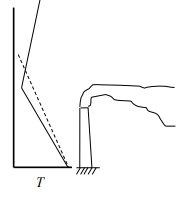
\includegraphics[width=0.2\columnwidth]{figs/oa.png}
  \caption{Option A}
  \label{fig:oa}
\end{figure} 
\item  \begin{figure}[H]
  \centering
  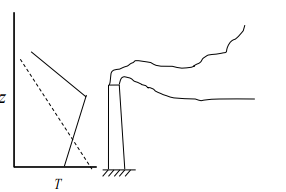
\includegraphics[width=0.2\columnwidth]{figs/ob.png}
  \caption{Option B}
  \label{fig:ob}
\end{figure}
\item   \begin{figure}[H]
  \centering
  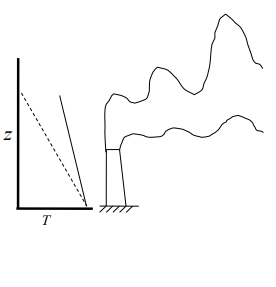
\includegraphics[width=0.2\columnwidth]{figs/oc.png}
  \caption{Option C}
  \label{fig:oc}
\end{figure} 
\item  \begin{figure}[H]
  \centering
  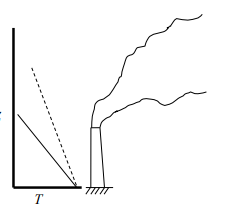
\includegraphics[width=0.2\columnwidth]{figs/od.png}
  \caption{Option D}
  \label{fig:od}
\end{figure}
  \end{enumerate}
\end{multicols}
\item The inventory pattern shown does NOT represent the following.
\begin{figure}[H]
  \centering
  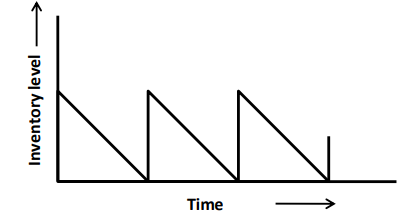
\includegraphics[width=0.2\columnwidth]{figs/invent.png}
  \caption{Graph}
  \label{fig:i}
\end{figure}

\hfill\brak{GATE\ MN\ 2018}
\begin{multicols}{2}
\begin{enumerate}
\item Inventory is replenished instantaneously
\item Demand decreases with time
\item Shortage is not permitted
\item Demand is uniform
\end{enumerate}
\end{multicols}
\item The figure depicts a transportation problem along with the solution. The correct statement is

\hfill\brak{GATE\ MN\ 2018}
\begin{figure}[H]
  \centering
  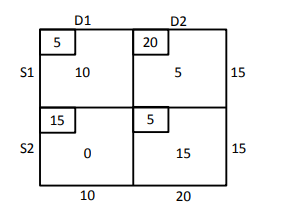
\includegraphics[width=0.4\columnwidth]{figs/fig.png}
  \caption{transportation problem }
  \label{fig:t}
\end{figure}
\begin{multicols}{2}
\begin{enumerate}
\item unbalanced problem, optimal solution
\item unbalanced problem, sub-optimal solution
\item balanced problem, optimal solution
\item balanced problem, sub-optimal solution
\end{enumerate}
\end{multicols}
\item The degree of the differential equation $\dfrac{d^{2}x}{dt^{2}} + 2x^{3} = 0$ is

\hfill\brak{GATE\ MN\ 2018}
\item The slope of the line connecting the points $\brak{20,6}$, $\brak{40,8}$,

\hfill\brak{GATE\ MN\ 2018}

\item  Two contours of RL $60$ m and $70$ m are separated by $34$ m measured along dip of the seam.The dip of the seam in degree is

\hfill\brak{GATE\ MN\ 2018}
\item The RL of the initial station is $200 \, \text{m}$. If $\sum BS = 1.54 \, \text{m}$ and $\sum FS = 0.45 \, \text{m}$, then the RL of the last station in m is 

\item For the conveyor belt drive shown, the tension on the tight side $(T_1)$ is double that of the slack side. The coefficient of friction between belt and drum is $0.21$. The minimum angle of lap (in degree) to avoid slippage of the belt is

\hfill\brak{GATE\ MN\ 2018}

\begin{figure}[H]
  \centering
  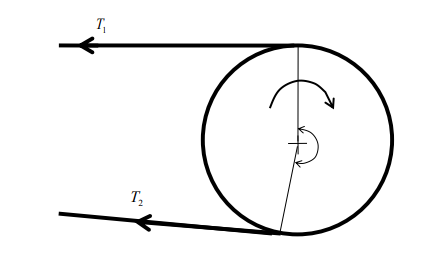
\includegraphics[width=0.4\columnwidth]{figs/figure.png}
  \caption{Schematic diagram of a pulley system}
  \label{fig:figure}
\end{figure}

\item In a bord and pillar development district, 6 headings driven along the strike direction are
surrounded by panel barriers on the dip and rise sides. The maximum possible number of faces for the panel is

\hfill\brak{GATE\ MN\ 2018}
\item A roadway in a mine, a single light source as shown, emits light uniformly in all directions. The floor level illumination at station A is $20$ lux. The floor level illumination at a point B in lux is 
\begin{figure}[H]
  \centering
  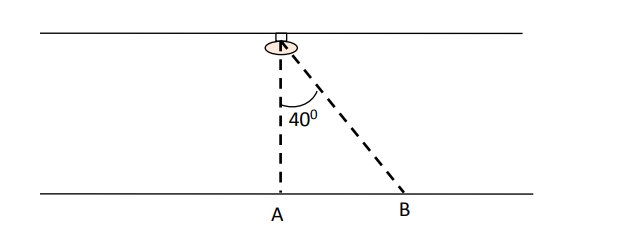
\includegraphics[width=0.4\columnwidth]{figs/source.png}
  \caption{Light Source}
  \label{fig:Ls}
\end{figure}
\hfill\brak{GATE\ MN\ 2018}
\item A system of two identical components connected in series has reliability of $0.25$. The reliability of each component is
\hfill\brak{GATE\ MN\ 2018}

\item The operational status of an HEMM in a shift is shown in the diagram. The availability of
the machine in \% is
\begin{figure}[H]
  \centering
  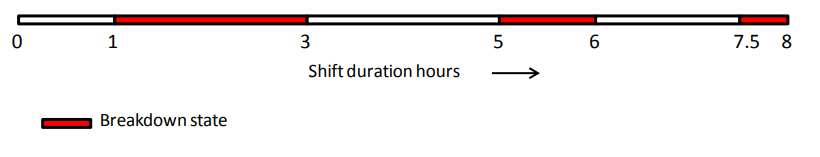
\includegraphics[width=0.4\columnwidth]{figs/HEMM.png}
  \caption{HEMM}
  \label{fig:HEMM}
\end{figure}
\hfill\brak{GATE\ MN\ 2018}

\item If $c$ is a constant, the solution of the differential equation $4y\dfrac{dy}{dx}+9x=0$ is  

\hfill\brak{GATE\ MN\ 2018}
\begin{multicols}{4}
\begin{enumerate}
\item $\dfrac{x^2}{81}+\dfrac{y^2}{16}=c$
\item $\dfrac{x^2}{16}+\dfrac{y^2}{81}=c$
\item $\dfrac{x^2}{9}+\dfrac{y^2}{4}=c$ 
\item $\dfrac{x^2}{4}+\dfrac{y^2}{9}=c$
\end{enumerate}
\end{multicols}

\item Match the following blasting elements with the corresponding initiators
\begin{table}[H]
  \centering
  \caption{Match The Following}
  \begin{tabular}{>{\bfseries}l l}
Specification & Outer Diameter in mm \\
P. AW & p. 34.9 \\
Q. BW & q. 44.4 \\
R. EW & r. 54.0 \\
S. NW & s. 66.7 \\
\end{tabular}


  \label{tab:Table1}
\end{table}

\hfill\brak{GATE\ MN\ 2018}
\begin{multicols}{4}
\begin{enumerate}
\item P-2, Q-3, R-4, S-1
\item P-3, Q-1, R-4, S-2
\item P-3, Q-1, R-2, S-4 
\item P-1, Q-4, R-2, S-3
\end{enumerate}
\end{multicols}

\item The following plot is developed for a rock type after a series of triaxial tests. The uniaxial
compressive strength and tensile strength of the rock type, respectively, in MPa, are

\hfill\brak{GATE\ MN\ 2018}
\begin{figure}[H]
  \centering
  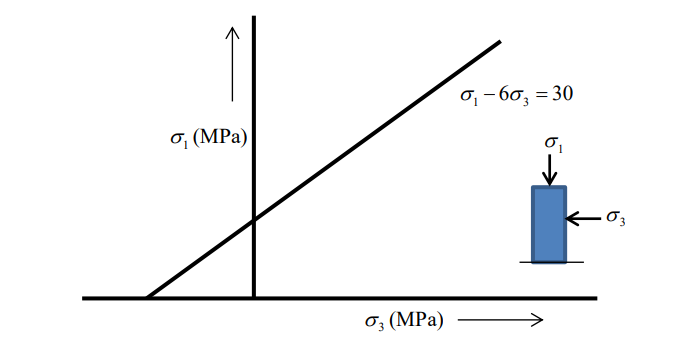
\includegraphics[width=0.4\columnwidth]{figs/graph1.png}
  \caption{graph}
  \label{fig:g1}
\end{figure}
\begin{multicols}{4}
\begin{enumerate}
\item $30,5$
\item $30,6$
\item $24,6$
\item $24,5$
\end{enumerate}
\end{multicols}

\item Match the following in the context of environmental management.
\begin{table}[H]
  \centering
  \caption{Match The Following}
  \begin{center}
\begin{tabular}{|c|c|c|c|c|c|}
\hline
Mass of particles, g      & 2   & 5   & 7   & 4   & 1    \\
\hline
Mean size of particles, $\mu$m & 350 & 240 & 200 & 150 & 100 \\
\hline
\end{tabular}
\end{center}
  \label{tab:Table2}
\end{table}

\hfill\brak{GATE\ MN\ 2018}
\begin{multicols}{4}
\begin{enumerate}
\item P-1, Q-4, R-3, S-2
\item P-3, Q-1, R-4, S-2
\item P-4, Q-3, R-1, S-2 
\item P-3, Q-4, R-1, S-2
\end{enumerate}
\end{multicols}

\item  A panel in coal mine produces $400$ tonne per day. The number of persons employed in each of the three shifts is $110$, $130$ and $120$. As per CMR, the minimum quantity of air that needs to be circulated at the last ventilation connection of the panel in $m^3
/min$ is

\hfill\brak{GATE\ MN\ 2018}
\begin{multicols}{4}
\begin{enumerate}
\item $780$
\item $900$
\item $1000$
\item $2400$
\end{enumerate}
\end{multicols}

\item A right conical iron ore stack on level ground of height 10 m has 60\% Fe. The height of the conical stack is extended up to 20 m using iron ore of 50\% Fe. The angle of repose of iron ore is $38^\circ$.The mean grade of the final stack in % Fe is
\hfill\brak{GATE\ MN\ 2018}

\item The feasible region of a linear programming problem is shown in the figure. The maximum value of the objective function $Z=4X+3Y$ is 
\begin{figure}[H]
  \centering
  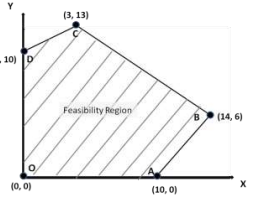
\includegraphics[width=0.4\columnwidth]{figs/LP.png}
  \caption{LP}
  \label{fig:LP}
\end{figure}
\hfill\brak{GATE\ MN\ 2018}


\item Cash flow of a project of duration 4 years is shown. The uniform income `R`, in Rs. crores, 
at the end of $2^{\text{nd}}$, $3^{\text{rd}}$ and $4^{\text{th}}$ years for an internal rate of return of 10\% is
\begin{figure}[H]
  \centering
  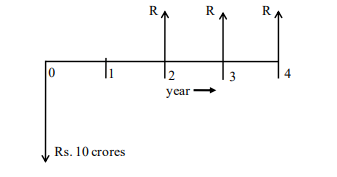
\includegraphics[width=0.4\columnwidth]{figs/Graph2.png}
  \caption{Graph}
  \label{fig:g2}
\end{figure}

\hfill\brak{GATE\ MN\ 2018}

\item The grade values of alumina at three sample locations \brak{A, B and C} in a bauxite 
deposit are as shown. Using the `inverse distance' method, the computed grade  in \% alumina at location Z is


\hfill\brak{GATE\ MN\ 2018}
\begin{figure}[H]
  \centering
  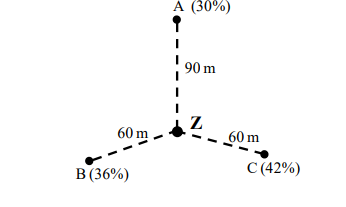
\includegraphics[width=0.4\columnwidth]{figs/figure1.png}
  \caption{Diagram}
  \label{fig:figure1}
\end{figure}

\item Economic feasibility of two methods is examined for meeting a targeted mine production. On a yearly basis, the following cost parameters (Rs in crores) are applicable for these methods.
\begin{table}[H]
  \centering
  \caption{Match The Following}
  \begin{table}[ht]
\centering
\begin{tabular}{|l|l|}
\hline
\textbf{Column I} & \textbf{Column II} \\ \hline
P. Hydraulic Conductivity   & 1. Upper limit of moisture available to plant \\ \hline
Q. Permeability            & 2. All soil pores are filled with water         \\ \hline
R. Viscosity               & 3. Soil capillarity                            \\ \hline
S. Surface Tension         & 4. Properties of fluid as well as soil          \\ \hline
T. Saturation Capacity     & 5. Property of the medium                      \\ \hline
U. Field Capacity          & 6. Internal friction that brings about resistance to flow \\ \hline
\end{tabular}
\end{table}
  \label{tab:Table3}
\end{table}
The annual rate of production, X in million tonnes for which both the methods will yield the same operating cost is 

\hfill\brak{GATE\ MN\ 2018}

\item A person standing $50$ m away from an HEMM experiences $90$ dB sound pressure level. If the person moves to a new location that is $70$ m away from the HEMM, the sound pressure level experienced by the person, in dB, becomes 

\hfill\brak{GATE\ MN\ 2018}
\item A portion of a ventilation system has two splits as shown. Split A has a resistance of $0.2$ $Ns^{2}/m^{8}$
and a regulator of size $2.0$ $m^2$. The resistance of split B in $Ns^{2}/m^{8}$ is
\begin{figure}[H]
  \centering
  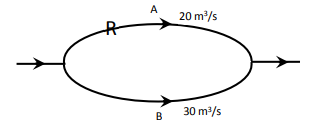
\includegraphics[width=0.4\columnwidth]{figs/figure2.png}
  \caption{Diagram}
  \label{fig:figure2}
\end{figure}

\hfill\brak{GATE\ MN\ 2018}
\item Air enters a bord and pillar panel at 10 ppm $CO$  and $20.78$\% $O_2$. The air at the panel return
has $80$ ppm $CO$ and $20.52$\% $O_2$. The Grahams ratio for the status of fire in the panel
in \% is $\colon$ 

\hfill\brak{GATE\ MN\ 2018}
\item In a sublevel stope, $20$ m high excavation is made with ring drilling in a $6$ m wide orebody.In an effective shift time of $6$ hrs, three rings are blasted resulting in $9$ m extraction length.LHDs of $5.0$ $m^3$ bucket capacity and cycle time of $5$ minutes are used for ore transportation. The number of LHDs required for this operation is
\hfill\brak{GATE\ MN\ 2018}
\item A coal seam lying at a depth of $200$ m is developed by bord and pillar method. Pillars are $30$ m centre to centre with a gallery width of $4$ m. Unit weight of the overlying strata is $28$ $kN/m^3$. If the pillar strength is $9.32$ MPa, the factor of safety of pillar is 

\hfill\brak{GATE\ MN\ 2018}

\item Following information about a longwall retreating panel is given.\\
Panel length = $1800$ m\\
Face length = $150$ m\\
Depth of web = $0.6$ m\\
Shearer travels at a speed of $1.5$ m/min along the face.
Each cutting cycle requires a non-operational time of $2$ h $20$ min. The panel is fully
extractable. The number of working days required to extract the panel is

\hfill\brak{GATE\ MN\ 2018}
\item In a direct rope haulage operating along a $1500$ m long incline, $180$ tonne of coal is hauled
in $7$ hours. The average rope speed is $7.5$ km/h. The set changing time for the tubs is $2$ minutes each at the top and bottom of the incline. If the tub capacity is $1.0$ tonne, the number of tubs in the set is

\hfill\brak{GATE\ MN\ 2018}.
\item An SDL of $1.0$ tonne capacity operates with a cycle time of $6$ minutes. The dimension of the face is $4$ m x $3$ m. Five blasts are conducted per shift with an average pull of $1.2$ m. If the density of blasted coal is $0.8$ $tonne/m^3$, the time required by the SDL in the shift to lift all the prepared coal in hours is

\hfill\brak{GATE\ MN\ 2018}

\item A force diagram is shown below. Considering clockwise moments to be positive, the resultant moment about A in Nm is
\begin{figure}[H]
  \centering
  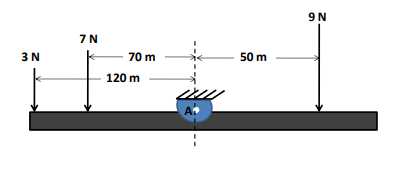
\includegraphics[width=0.4\columnwidth]{figs/force.png}
  \caption{Diagram}
  \label{fig:force}
\end{figure}


\hfill\brak{GATE\ MN\ 2018}
\item The experiment to determine permeability of a soil sample is illustrated below. The crosssectional area of the sample is $20.0$ $cm^2$ .The permeability of the soil sample in $cm/s$ is
\begin{figure}[H]
  \centering
  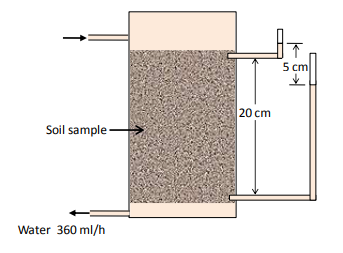
\includegraphics[width=0.4\columnwidth]{figs/ex.png}
  \caption{Diagram}
  \label{fig:eg}
\end{figure}

\hfill\brak{GATE\ MN\ 2018}

\item In underground face blasting, the pull is found to be $10$\% less than the drillhole length. The headings of $3.6$ m width are supported by prop density of $1.44$/$m^2$.The hole length is $1.5$ m, and $6$ rounds of blasting are done in the panel per shift. The number of props to be erected in a shift is

\hfill\brak{GATE\ MN\ 2018}
\item The immediate roof of a mine is supported by bolts of length 1.5 m, arranged in $1.2$ m x $1.2$ m grid pattern. If the unit weight of roof rock is $2.25$ $tonne/m^3$ and load carrying capacity of each bolt is $7.5$ tonne, the factor of safety of the support system is

\hfill\brak{GATE\ MN\ 2018}
\item In a level terrain, a vertical orebody of $20$ m uniform width is worked by surface mining method. The density of the ore is $2.5$ $tonne/m^3$.The ultimate pit has a depth of $60$ m, width of $20$ m at pit bottom, and a pit slope of $45^\circ$.The overall stripping ratio for this condition in $m^3 /tonne$ is 

\hfill\brak{GATE\ MN\ 2018}
\item A $20$ m long steel tape used for survey is found to be short by $10$ cm. If the area measured with the steel tape is $5000$ $m^2$,the actual area in $m^2$ is

\hfill\brak{GATE\ MN\ 2018}
\item The following figure shows the designed blast pattern of a bench. The explosive column is charged at $18$ $kg/m$. If the unit weight of the blasted material is $2.5$ $tonne/m^3$,the powder factor for the blast in tonne/kg is
\begin{figure}[H]
  \centering
  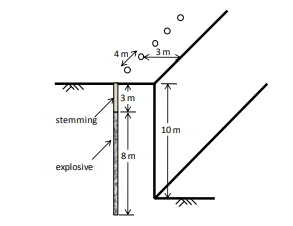
\includegraphics[width=0.4\columnwidth]{figs/pattern.png}
  \caption{Diagram}
  \label{fig:pattern}
\end{figure}

\hfill\brak{GATE\ MN\ 2018}


\item Two points on the equator have longitudes $55^\circ E$ and $25^\circ W$. Considering radius of earth as $6400$ km, the distance between the two points in km is

\hfill\brak{GATE\ MN\ 2018}
\item Sum of the series $5$,$10$, $15$,   , $500$ is 

\hfill\brak{GATE\ MN\ 2018}
\item The sample standard deviation for the following set of observations is $40$, $45$, $50$ and $55$

\hfill\brak{GATE\ MN\ 2018}
\item For the given function $f(x,y) = (3+x)(4+y)$, the value of 
$\dfrac{\partial f}{\partial x} + \dfrac{\partial f}{\partial y}$ 
at $x=2$ and $y=1$ is \underline{\hspace{2cm}}.


\hfill\brak{GATE\ MN\ 2018}
\item A positive integer $m$ in base 10, when represented in base 2 has the representation $p$, and in base 3 has the representation $q$. We get $p - q = 990$, where the subtraction is done in base 10. Which of the following is necessarily true $\colon$

\hfill\brak{GATE\ MN\ 2018}
\item Given $y = x^2 + x + 6$, the value of $\dfrac{d}{dx}(\ln y)$ at $x=2$ is \underline{\hspace{2cm}}.
\hfill\brak{GATE\ MN\ 2018}
\begin{center}
\Large\textbf{{END OF THE QUESTION PAPER}}
\end{center}
\end{enumerate}

\end{document}





